\documentclass{beamer}
\usepackage[polish]{babel}

% \usepackage{polski}
%%%%%%%%% tu zmieniałam:
\usepackage[utf8]{inputenc} % język
\usepackage[T1]{fontenc} % język
\usepackage{epsfig} % do obsługi eps
\usepackage{epstopdf} % do obsługi eps

\usepackage{ragged2e} % do justowania
%%%%%%%%% dotąd
\usepackage{listings}

\colorlet{structure}{red!65!black}

\beamertemplateshadingbackground{white}{white}

\usepackage{beamerthemesplit}
\usepackage{graphics}
\usepackage{graphicx}
\usepackage{hyperref}

\title{Symulacja rynku spożywczego: postępy prac}
\author{Beata Wójciak, Weronika Świderska}
\date{Wrocław, \today}


\begin{document}
	\frame { \titlepage }

\frame{
 \justifying 
 W~naszym projekcie planujemy stworzyć system złożony z~agentów symulujących
zachowanie uczestników rynku żywieniowego. 

Każdy z~agentów będzie działał według własnego schematu.
\frametitle{Modelowanie zachowania rynku}
}

\frame {
\frametitle{Agenci i relacje między nimi}
	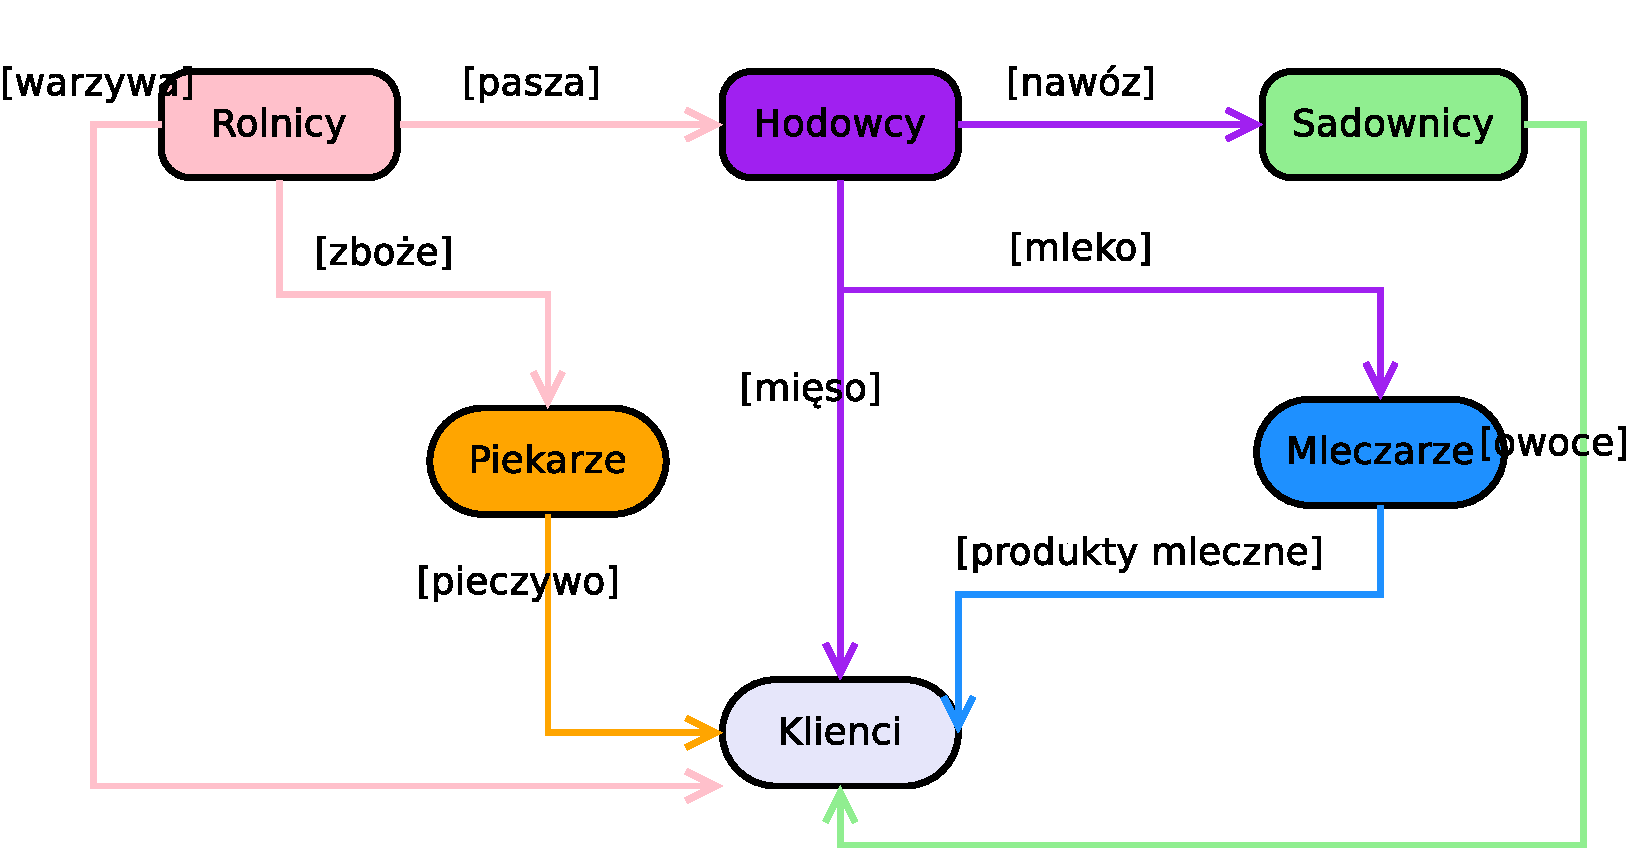
\includegraphics[scale=0.4]{diagram_kolorowy.eps}

}
\frame {
\frametitle{Co zostało wykonane}
	\begin{itemize}
	\item Zostały wyspecyfikowane relacje pomiędzy poszczególnymi typami agentów
	\item Zostały ustalone jednostki~i zależności między jednostkami dla każdego typu produktu
	\item Powstała implementacja interfejsu systemu oraz bazowe funkcjonalności agentów
	\end{itemize}
}

\frame {
\frametitle{Szczegóły}
	\begin{itemize}
	\item Symulacja napisana jest~w Javie~z wykorzystaniem JADE'a
	\item Każdy rodzaj transakcji jest osobną rozmową
	\item Obecnie agenci widzą się nawzajem~i~w ograniczonym zakresie komunikują ze sobą
	\item Każdy agent dziedziczy po agencie bazowym, co ułatwia implementację
	\end{itemize}
}

\frame {
\frametitle{Co należy jeszcze wykonać}
	\begin{itemize}
	\item Dokończyć implementację agentów
	\item Przetestować aplikację dla różnych wartości parametrów
	\end{itemize}
}
\frame {
\frametitle{Parametry agentów: rolnicy}
Początkowo dostają:
	\begin{itemize}
	\item Określoną liczbę jednostek pól (losowo między 200~--~1000)
	\item Określoną ilość ziarna (losowo tak, aby być w stanie obsiać co najmniej pół pola)
	\item Losową ilość pieniędzy z zakresu (100~--~400)
	\end{itemize}
Założenia:
	\begin{itemize}
	\item Nie mogą sprzedawać całego zboża, bo jest im potrzebne do siewu~---~zostawiają sobie co najmniej tyle, by móc obsiać połowę pola
	\item Potrzebują pieniędzy na zakup nowych pól oraz nawozu
	\item Mogą przechowywać zboże na przyszłość
	\end{itemize}
}

\frame {
\frametitle{Parametry agentów: hodowcy}
Początkowo dostają:
	\begin{itemize}
	\item Określoną liczbę zwierząt (losowo między 5-20)
	\item Losową ilość pieniędzy z zakresu (100~--~400)
	\end{itemize}
Założenia:
	\begin{itemize}
	\item Nie wybijają więcej niż połowy początkowej liczby zwierząt
	\item Potrzebują pieniędzy na zakup nowych zwierząt i ziarna
	\item Zwierzęta produkują mleko, nawóz i mięso
	\end{itemize}
}

\frame {
\frametitle{Parametry agentów: piekarze i mleczarze}
Początkowo dostają:
	\begin{itemize}
	\item Określoną liczbę pracowników (losowo między 1-10)
	\item Losową ilość pieniędzy z zakresu (100~--~400)
	\end{itemize}
Założenia:
	\begin{itemize}
	\item Produkcja zależy od liczby pracowników
	\item Dochód jest pomniejszany o pensję dla pracowników
	\item Piekarz może przechowywać zboże
	\item Mleczarz nie może przechowywać mleka
	\end{itemize}
}

\frame {
\frametitle{Parametry agentów: sadownicy}
Początkowo dostają:
	\begin{itemize}
	\item Określoną liczbę jednostek pól (losowo między 100~--~500)
	\item Losową ilość pieniędzy z zakresu (100~--~400)
	\end{itemize}
Założenia:
	\begin{itemize}
	\item Pieniądze potrzebują na zakup pola, nawozu i nowych drzew
	\item Część owoców zachowują dla siebie 
	\end{itemize}
}

\frame {
\frametitle{Parametry agentów: klienci}
Początkowo dostają:
	\begin{itemize}
	\item Losową ilość pieniędzy z zakresu (1300~--~4000)
	\end{itemize}
Założenia:
	\begin{itemize}
	\item W ciągu miesiąca robią zakupy 4 razy
	\item Zapotrzebowanie na produkty pozostaje stałe
	\item Nic nie produkują
	\end{itemize}
}

\frame {
\begin{center}
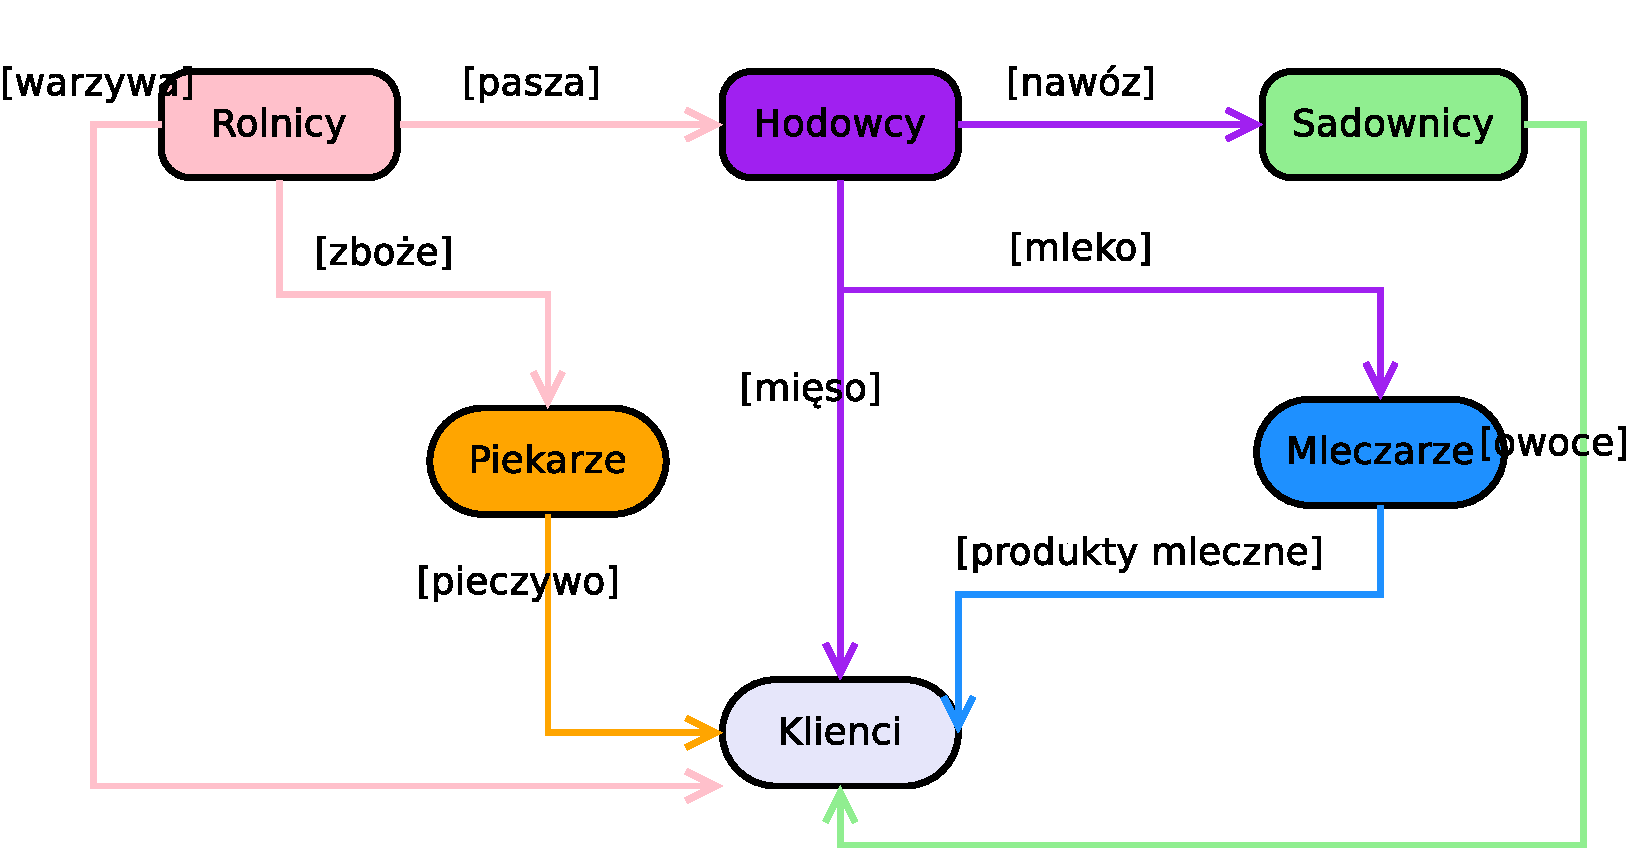
\includegraphics[scale=0.4]{diagram_kolorowy.eps}
\end{center}
}
\end{document}